\chapter{Results and Discussion}

Here we examine both the performance and visual quality of our global illumination algorithm. The primary means of evaluating performance is based on frame time. The times of each render pass are recorded as well as a total frame time. Evaluating visual quality is based largely on whether the lighting appears smooth and believable with a minimal amount of noise and artifacts.

We also discuss the application of voxel warping and how it compares with other global illumination methods. Unfortunately, direct performance and visual quality comparisons are difficult to objectively measure as there are many contributing factors---mesh complexity and optimizations, texture resolution and format, shading model, graphics API, hardware, GPU driver version, and more---that affect the final comparison, in addition to the exact implementation details. Nevertheless, we provide motivations and tradeoffs between our method and others and their potential impact on performance and quality.

\section{Test Setup}
% TODO verify driver, kernel, resolution when getting final results
All results are obtained from a system with an i5-2400 CPU, 8GB of DDR3 RAM, and an NVIDIA GeForce GTX 970 GPU. The system is running Arch Linux kernel 4.16.8-1 and uses the proprietary NVIDIA graphics driver version 396.24. The application uses an OpenGL 4.5 context and the scene is rendered with a window resolution of 1920x1080.

% TODO give #vertices, texture resolutions and sizes?
The model used in the test scenes is the Crytek Sponza scene\footnote{The original Sponza model can be acquired from Crytek~\cite{sponza_og}. The model we use is modified by Alexandre Pestana~\cite{sponza_pbr}.}. The textures from the original Sponza scene are replaced with ones necessary for physically-based rendering (materials are defined by a diffuse color, roughness, metallic coefficient, normal, and optionally an alpha texture). Mipmaps for the original textures were also precomputed and stored along with the full size 1024x1024 textures as DDS (Microsoft DirectDraw Surface) files using the compressed DXT5 format for faster scene loading.

To measure performance timings for each render pass we make use of OpenGL timer queries using the \verb#GL_TIME_ELAPSED# query type. The results of the query object are double buffered to ensure introducing the timer query does not affect the total render time.

Unless otherwise mentioned, voxel resolutions are 256x256x256 with 6 mipmap levels.

\section{Analysis}
In the following sections we evaluate various aspects of our work. First, we discuss the global illumination algorithm as a whole. Second, we compare the rasterization-based and tessellation-based voxelization algorithms. Lastly, we provide the results of our voxel warping and some insights on future improvements.

\subsection{Global Illumination}
Table~\ref{tbl:renderpasstiming} shows timing results from the complete global illumination algorithm. We test the algorithm with different screen resolutions and voxel grid resolutions. Recall that a minimum goal for real-time is 30 frames per second and a target is 60 frames per second, which correspond to individual frame times of 33.3ms and 16.7ms, respectively. We see that the total frame time always meets the goal of 60 frames per second.

The data shows that shadowmap creation and radiance injection was independent of screen resolution and voxel resolution\footnote{As expected, since the main factor for both of these render passes is the size of the shadowmap, which remained constant at 4096x4096.}. The voxelization and radiance filtering steps both only depended on voxel grid resolution. The depth prepass also only varied with respect to screen resolution. The final shading predictably depended on both voxel grid resolution and screen resolution. However, larger voxel grid resolutions did not affect the final shading times by much at a given screen resolution, with approximately a 1.5ms difference between using a voxel resolution of 64 versus 256.

\begin{table}[H]
\centering
\begin{tabular}{l ccc ccc ccc}
\toprule
Render Pass & \multicolumn{9}{c}{Render Pass Time (ms)} \\
& \multicolumn{3}{c}{1280x720} & \multicolumn{3}{c}{1600x900} & \multicolumn{3}{c}{1920x1080} \\
& 64 & 128 & 256 & 64 & 128 & 256 & 64 & 128 & 256 \\
\midrule
Voxelize           & 0.90 & 1.13 & 2.40  & 0.70 & 1.12 & 2.39  & 0.72 & 1.15 & 2.41\\
Shadowmap          & 0.69 & 0.69 & 0.69  & 0.69 & 0.69 & 0.69  & 0.68 & 0.68 & 0.69\\
Radiance Injection & 0.92 & 0.92 & 0.93  & 0.92 & 0.92 & 0.93  & 0.92 & 0.92 & 0.93\\
Radiance Filtering & 0.04 & 0.10 & 0.55  & 0.05 & 0.10 & 0.56  & 0.04 & 0.10 & 0.55\\
Depth Prepass      & 0.20 & 0.20 & 0.20  & 0.25 & 0.26 & 0.25  & 0.31 & 0.31 & 0.36\\
Final Shading      & 3.89 & 4.81 & 5.32  & 5.98 & 6.42 & 7.10  & 8.23 & 9.40 & 9.75\\
\midrule
Total              & 7.02 & 8.21 & 11.12  & 9.46 & 10.15 & 13.43  & 11.23 & 12.83 & 16.31\\
\bottomrule
\end{tabular}
\caption{Times measured for each render pass for various screen resolutions and voxel grid resolutions. The total timer also accounts for any other operations performed within each frame (i.e.\ the sum of the render pass times is not necessarily the complete time for an entire frame). Voxelization is done using the tessellation-based approach.}
\label{tbl:renderpasstiming}
\end{table}

\subsection{Tessellated Voxelization}
In terms of both performance and visual quality both voxelization methods are very similar. Voxelization times for each method are shown in Table~\ref{tbl:voxelizationtiming}, where we see the tessellation-based voxelization is slightly slower than the rasterization-based approach\footnote{However both implementations were not heavily optimized.}. Figure~\ref{fig:results_voxelization} compares the final rendered scene with both voxelization methods. The differences are minor.

Ultimately, both voxelization methods are sufficient for real-time global illumination. The (unoptimized) tessellation-based approach is slightly easier to implement and debug\footnote{Since the voxels are written in the tessellation evaluation stage, it is simple to add a geometry shader that takes the vertices and expands them into cubes, which are then rasterized and shaded with the vertex color (the same color inserted into the voxel texture).} but is slower than the rasterization-based approach. Also, since the rasterizer is not used, finding the dominant axis and conservative rasterization are not required with the tessellation-based approach. % One benefit of the tessellation-based approach is the voxel positions are continuous, unlike the rasterized voxels which are fixed at discrete positions according to the viewport resolution. This eliminates having to deal with cracks caused by higher density areas. (instead the limitation is on # of tesslevels ...)

\begin{figure}[h!]
\centering
    \begin{subfigure}[t]{0.4\textwidth}
        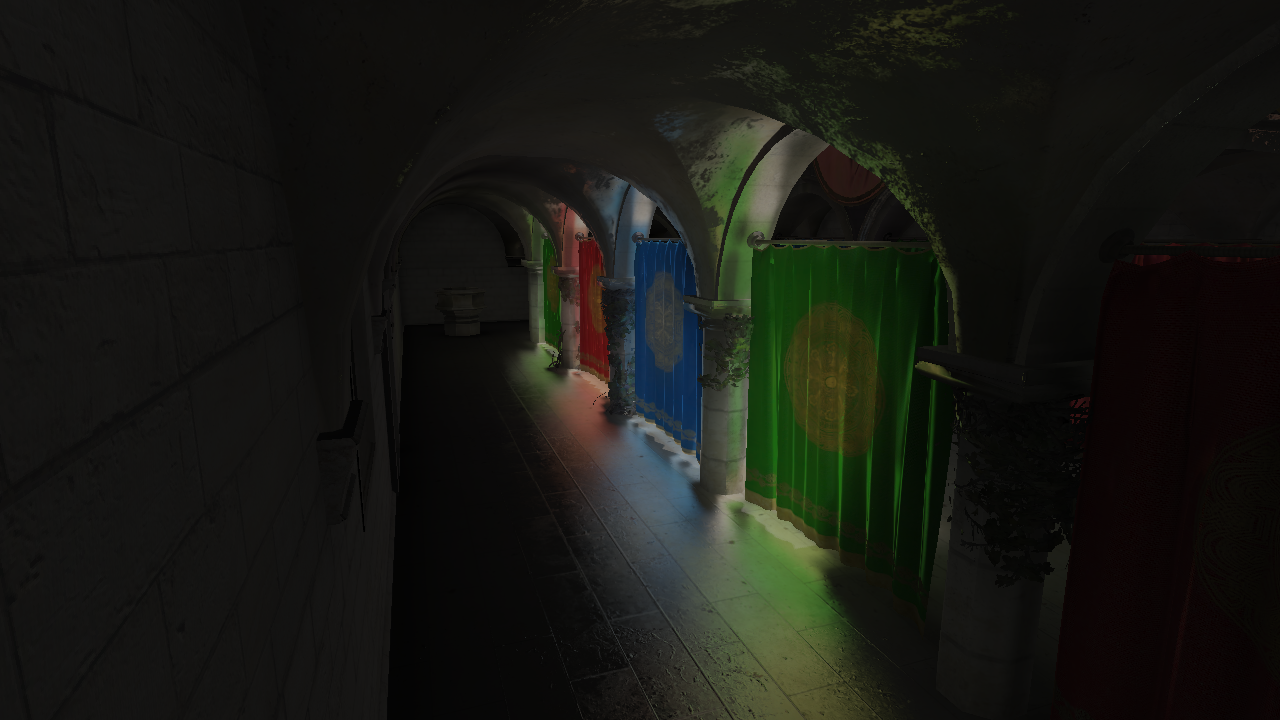
\includegraphics[width=\textwidth]{results_voxelraster.png}
        \caption{Rasterized voxels}
    \end{subfigure}
    ~
    \begin{subfigure}[t]{0.4\textwidth}
        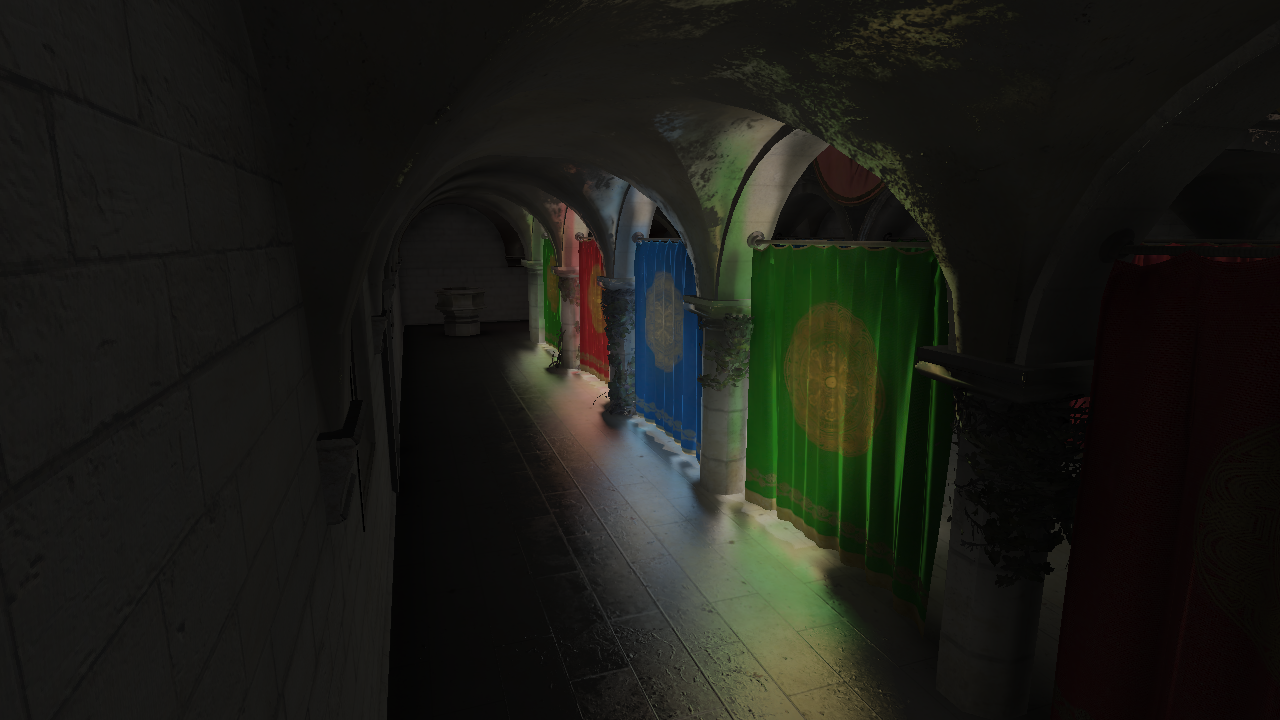
\includegraphics[width=\textwidth]{results_voxeltess.png}
        \caption{Tessellated voxels}
    \end{subfigure}
    \caption{The final rendered image for both voxelization methods have negligable visual differences.}
    \label{fig:results_voxelization}
\end{figure}

\begin{table}[H]
\centering
\begin{tabular}{lcc}
\toprule
\multirow{2}{*}{Voxel Grid Size} & \multicolumn{2}{c}{Voxelization Time (ms)} \\
& Rasterization-Based & Tessellation-Based \\
\midrule
64x64x64        & 0.53 & 0.70\\
128x128x128     & 0.85 & 1.12\\
256x256x256     & 1.91 & 2.35\\
\bottomrule
\end{tabular}
\caption{Time spent voxelizing the scene with varying voxel grid resolutions. For the rasterization-based approach the MSAA method of conservative rasterization is used.}
\label{tbl:voxelizationtiming}
\end{table}

\subsection{Integration of Voxel Cone Tracing into Existing Engines}
Voxel cone tracing is an attractive method for adding full global illumination to existing engines. The necessary information needed for the algorithm should already be available in most engines. A voxelized representation of the scene can be generated from any arbitrary triangle mesh using either of the voxelization methods presented. Other methods for voxelization could also be used if, for example, some geometry is generated procedurally. For radiance injection the only external inputs required are shadowmaps (or RSMs) for any lights that will contribute to the indirect lighting. Finally, the cone tracing needs surface normals and a TBN matrix (to transform the cone directions to world space), which will already be available for any engine which supports normal mapping.

\subsection{Voxel Warping}
Recall that the goal of voxel warping is to achieve a nonuniform voxel density. Ideally, this results in finer lighting detail for those areas that have increased density. Other approaches to increasing voxel resolution include clipmaps and octrees, as discussed in the Related Works. Fundamentally, however, the voxel resolutions were restricted to fixed sizes. With voxel warping we investigated how lifting this restriction would affect the voxelization quality.

The first method of voxel warping used a warp function to adjust the voxel density based on distance from the camera. Figure~\ref{fig:results_warpslope} shows a visual representation of the density. The effect of the warping on the final lighting is fairly minimal, see Figure~\ref{results_voxelwarp}. The big problem with voxel warping arises when the camera moves, since the continuously changing resolution causes voxels to flicker as they move throughout the voxel grid. Typically when the voxel sizes are all uniform this is fixed by snapping the voxel grid to discrete steps; but, with voxel warping, there is no single step size appropriate for all voxels.

\begin{figure}[h!]
    \centering
    
\includegraphics[width=\textwidth]{voxelwarp_slope.png}
    \caption{The scene is colored based on its density along the x axis (derived from the gradient of the warp function). Blue tints correspond to a slope of 2 and green corresponds to a slope of 1 (same as no warping).}
    \label{fig:results_warpslope}
\end{figure}

\begin{figure}[h!]
    \centering
    \begin{subfigure}[t]{0.4\textwidth}
        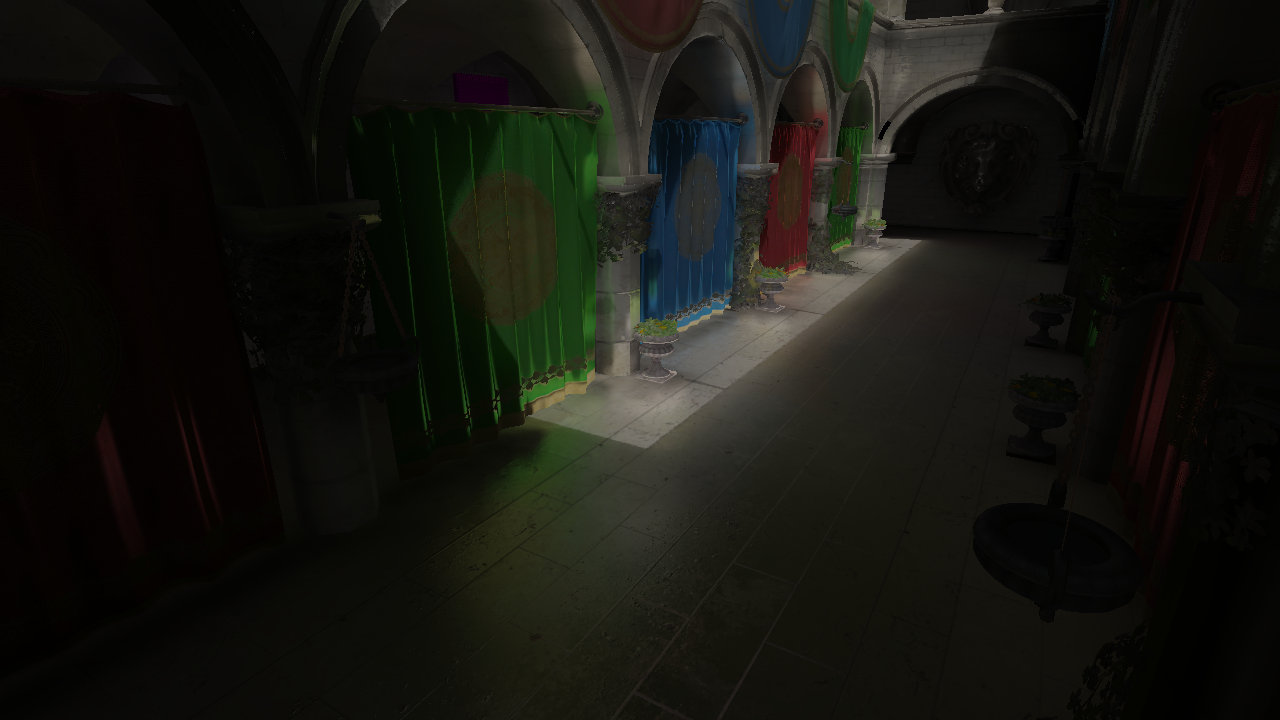
\includegraphics[width=\textwidth]{voxelwarp_off.png}
        \caption{Without voxel warping}
    \end{subfigure}
    ~
    \begin{subfigure}[t]{0.4\textwidth}
        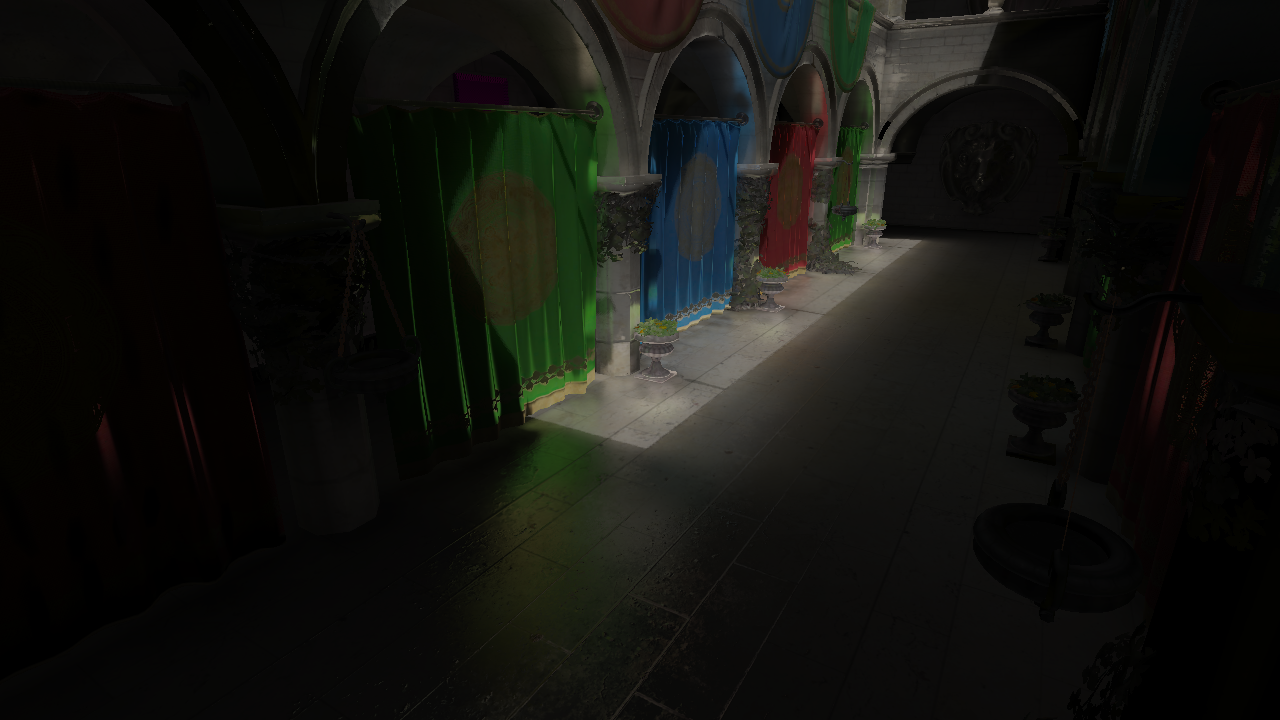
\includegraphics[width=\textwidth]{voxelwarp_on.png}
        \caption{With voxel warping}
    \end{subfigure}
    \caption{The voxel warping only has a small effect on lighting quality (the reflection of the green curtain is slightly more detailed).}
    \label{fig:results_voxelwarp}
\end{figure}

The second method of voxelization utilizes perspective projection to determine the voxel sizes. The motivation behind this is for voxel sizes to correspond to their respective size in screen space. The lighting quality for this approach is noticeably better than with the warp function, see Figure~\ref{fig:results_tesswarp}, however the temporal flickering issues are still apparent. With future work, we think this can be alleviated or eliminated.

\begin{figure}[h!]
    \centering
    \begin{subfigure}[t]{0.4\textwidth}
        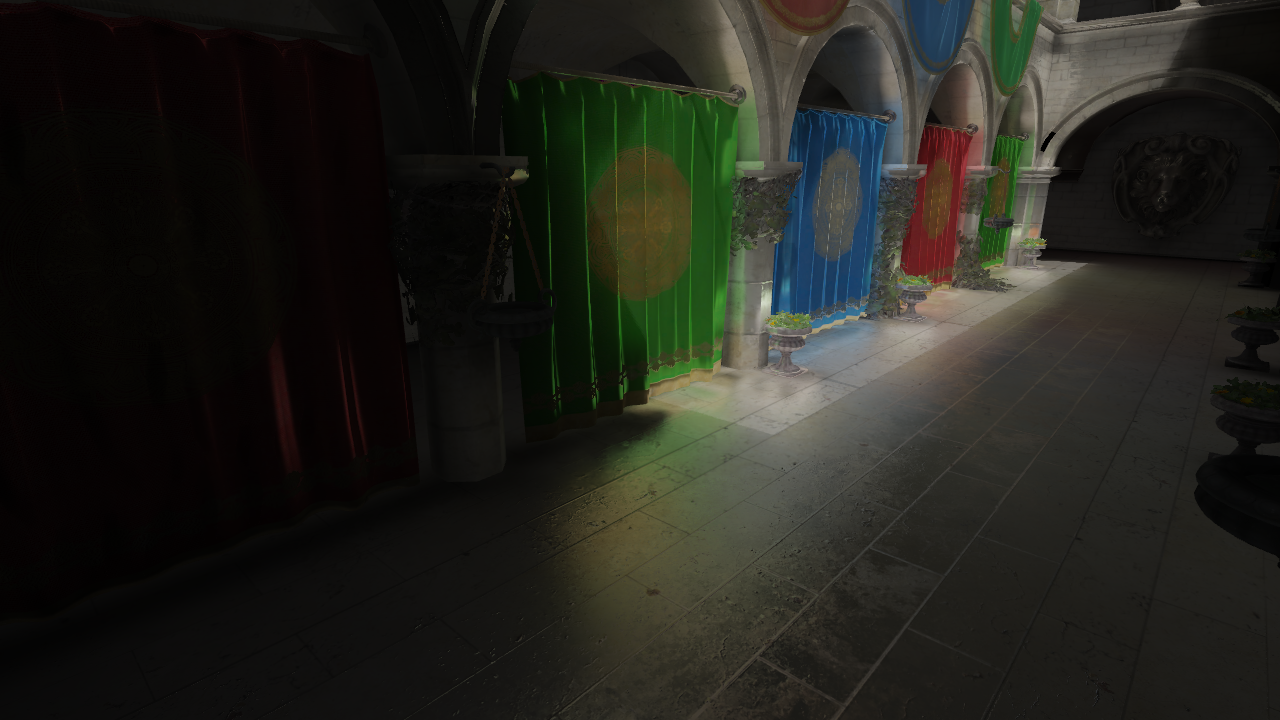
\includegraphics[width=\textwidth]{tesswarp_off.png}
        \caption{Without voxel warping}
    \end{subfigure}
    ~
    \begin{subfigure}[t]{0.4\textwidth}
        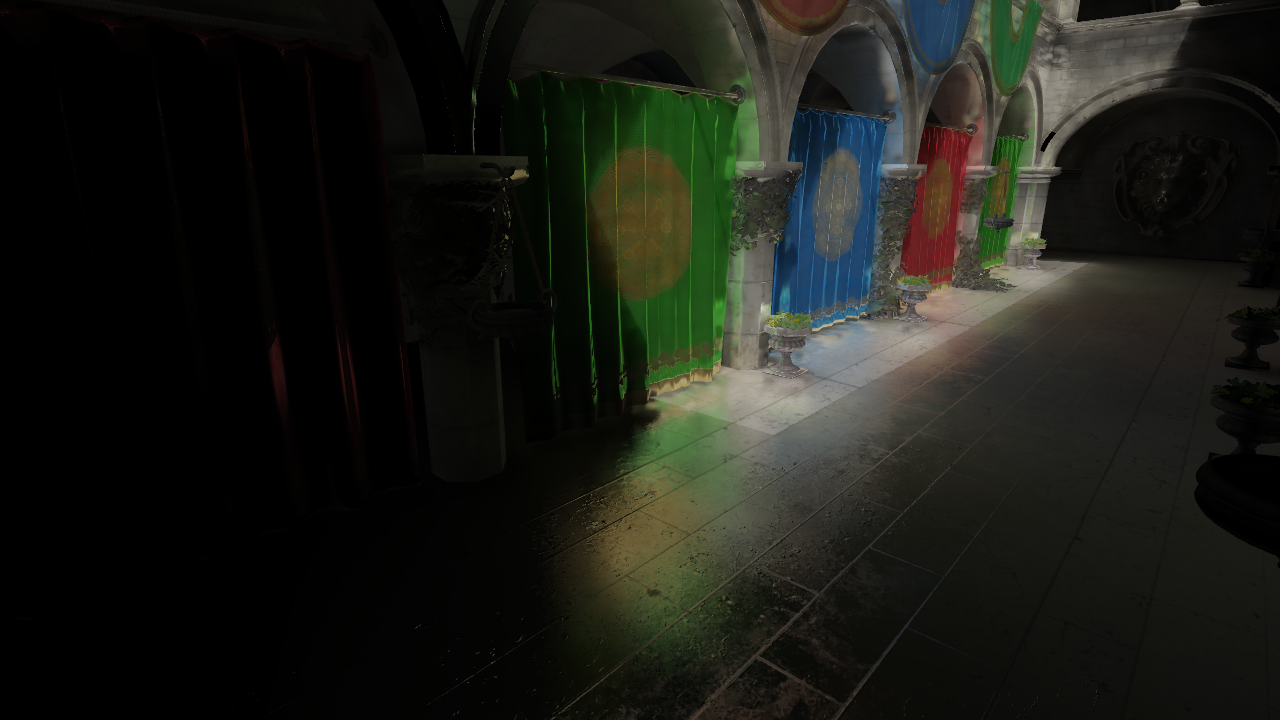
\includegraphics[width=\textwidth]{tesswarp_on.png}
        \caption{With voxel warping}
    \end{subfigure}
    \caption{The perspective voxel warping has a noticeable effect on lighting quality.}
    \label{fig:results_tesswarp}
\end{figure}

% atomicMax vs atomicAvg?
% warp textures? motivation was to not rely on camera for detail but base it on scene geometry. problem is finding good weights and moving objects causing those weights to change

% TODO other evaluations: GL_RGBA16F vs GL_RGBA8, comparison of conservative rasterization methods, comparison of filters, different cone weights/angles/directions?
% 2d from above view of voxel warp slope

\section{Conclusions}
In this work we implemented a real-time global illumination algorithm based on voxel cone tracing. We experimented with a tessellation-based voxelization method and nonuniform voxelization. Various aspects of our algorithm including performance and visual quality are evaluated and discussed. We find both rasterization-based and tessellation-based voxelization are similar in terms of both performance and voxelization quality. The voxel warping techniques provide promising results for further research. Most importantly, we provide a simple and cross platform implementation for future work.

\section{Future Work}
The goal of voxel warping was to increase voxel density for more detailed lighting as well as more efficiently use space within a 3D texture (and without the complexities of a sparse voxel octree). Unfortunately, having continuous voxel sizes makes minimizing temporal flickering difficult. To achieve the same goals while still having fixed voxel sizes, an approach to storing the voxels based on cascaded sparse 3D textures seems promising. Sparse textures (provided via the \verb#ARB_sparse_texture# extension for OpenGL) are analogous to classic virtual memory systems: not all parts of the texture are actually allocated in memory. Only the parts of the voxel texture that are used would require memory (of course the implementation allocates in fixed-size chunks, similar to pages in virtual memory). This approach would (ideally) combine the adaptive storage of octrees with the adaptive detail and hardware texture filtering of cascaded 3D textures.

% TODO solid voxelization?

For continued work on perspective voxel warping, exploring how to reduce temporal flickering would be worthwhile. Currently, voxels are aligned perpendicularly to the camera (a result of the view frustum having perpendicular near and far planes). Instead, having the voxels be curved may help reduce flickering when rotating the camera since the boundaries between adjacent voxels would be smooth. Essentially, the voxels would be described using spherical coordinates instead of cartesian coordinates.

Another potential area of improvement is alternative methods of storing radiance. For example, a spherical harmonics representation or ambient dice~\cite{iwanicki2017ambient} representation could be used. This would have impacts on both lighting quality, performance, and memory usage. In addition, the use of anisotropic methods to reduce light filtering through solid objects could also be added.

An interesting topic to explore in depth would be dynamically adjusting the cone tracing step based on factors such as local geometric surface complexity or distance from the camera. For example, Panteleev discusses computing indirect lighting at a reduced resolution and then interpolating the resulting lighting for smooth surfaces~\cite{practicalvxgi}. Interpolation was also used for RSMs to reduce the amount of computation~\cite{Dachsbacher:2005:RSM:1053427.1053460}. Other miscellaneous optimizations for voxel cone tracing could also be pursued, such as only updating subregions of the voxel volume or filtered radiance at a time~\cite{mclaren2016cascaded}.

% the real takeaways: warping is not a good idea due to temporal coherency issues. Using a cascaded approach with other clever tricks such as voxel culling, toroidal addressing, sparse textures/hybrid octree is a better approach.
% if i were to rewrite: voxelize only occupancy, use RSM to inject radiance (would like to test difference between a 'smart gather' where only filled voxels perform the gather and a scatter), anistropic voxel filtering, cascaded sparse 3d textures, ibl/environment map for outer edges, smarter filtering (gaussian w/ hole fill?)